\section{システムについて} 

\subsection{システムの動作要件} 本システムでは,ノートパソコンにLinuxサーバのセットアップを行い,サーバとして使用した. ネットワークは,学内の固定IPを割り当ててもらい,学内ネットワークを使用した. 
サーバのスペックは以下の通りである.
\subsubsection{サーバのスペック} 
\begin{itemize} 
\item OS: Ubuntu 22.04.3 LTS 
\item メモリ: 4GB 
\item CPU: Intel® Core(™) i7 
\item GPU: NVIDIA GeForce GTX 470M \item HDD: 80GB 
\end{itemize}
\subsection{システムの開発環境} 本システムの開発には,以下の言語やツールを使用した.
\subsubsection{使用言語} 
\begin{itemize} 
\item フロントエンド: 
\begin{itemize} 
\item html 
\item JavaScript 
\item css 
\end{itemize} 
\item バックエンド: 
\begin{itemize} 
\item JavaScript (Node.js) 
\item Python 
\end{itemize} 
\end{itemize}
\subsubsection{使用ツール} 
\begin{itemize} 
\item エディタ: VSCode 
\item ブラウザ: Google Chrome 119 
\end{itemize}
\subsection{システムの機能詳細} 本システムは,以下の3つの機能を提供する.
\subsubsection{電車の画像の分類} この機能では,ユーザがブラウザからアップロードした画像に含まれる電車の種類を分類する. 分類の結果,最も可能性が高いものをHTMLページに出力する.出力後の画面を\ref{電車の画像の分類}に示す 
\subsubsection{電車の画像の識別} この機能では,ユーザがブラウザからアップロードした画像に含まれる電車の位置と種類を識別する.  識別の結果,バウンディングボックスが追加された画像をHTMLページに表示する.出力後の画面を\ref{電車の画像の識別}に示す.
\subsubsection{電車の動画の識別} この機能では,ユーザがブラウザからアップロードした動画に含まれる電車の位置と種類を識別する. 識別の結果,バウンディングボックスが追加された動画をHTMLページに表示する.出力後の画面を\ref{電車の動画の識別}に示す.

\begin{figure}[htbp]
  \centering
  \begin{minipage}[t]{0.3\\textwidth}
    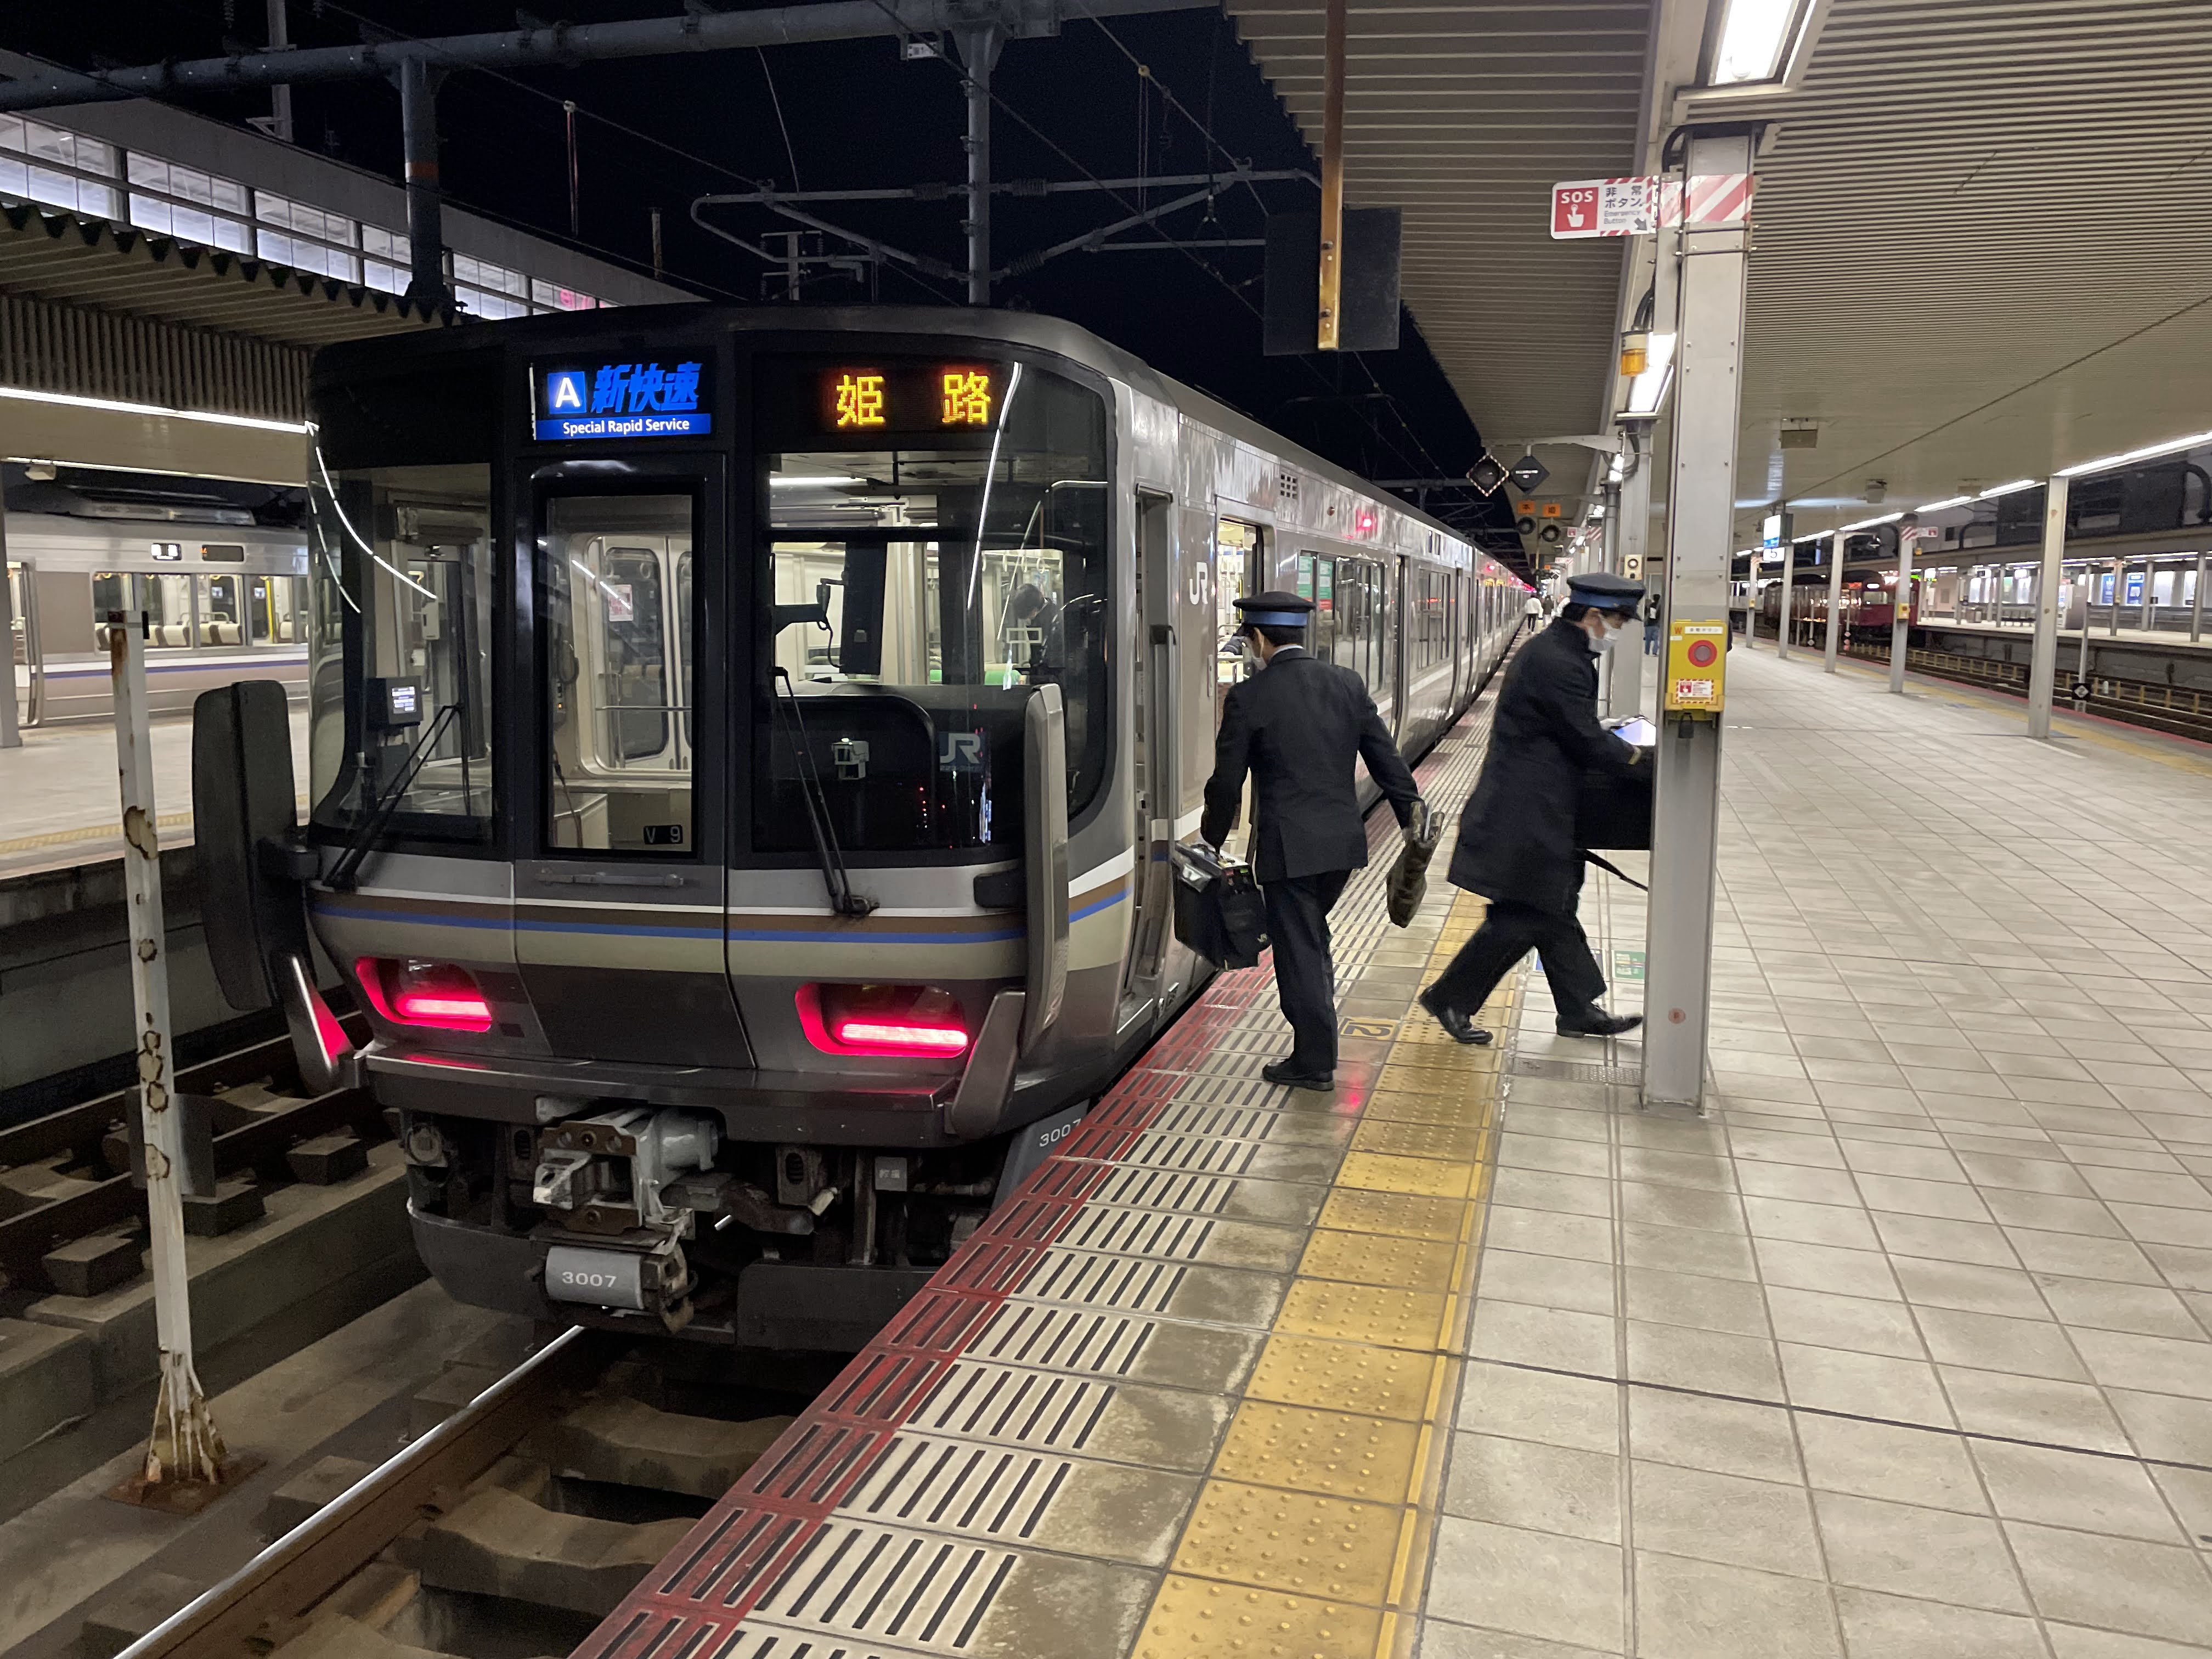
\includegraphics[width=\\linewidth]{image1.png}
    \caption{電車の画像の分類}
  \end{minipage}
  \hfill
  \begin{minipage}[t]{0.3\\textwidth}
    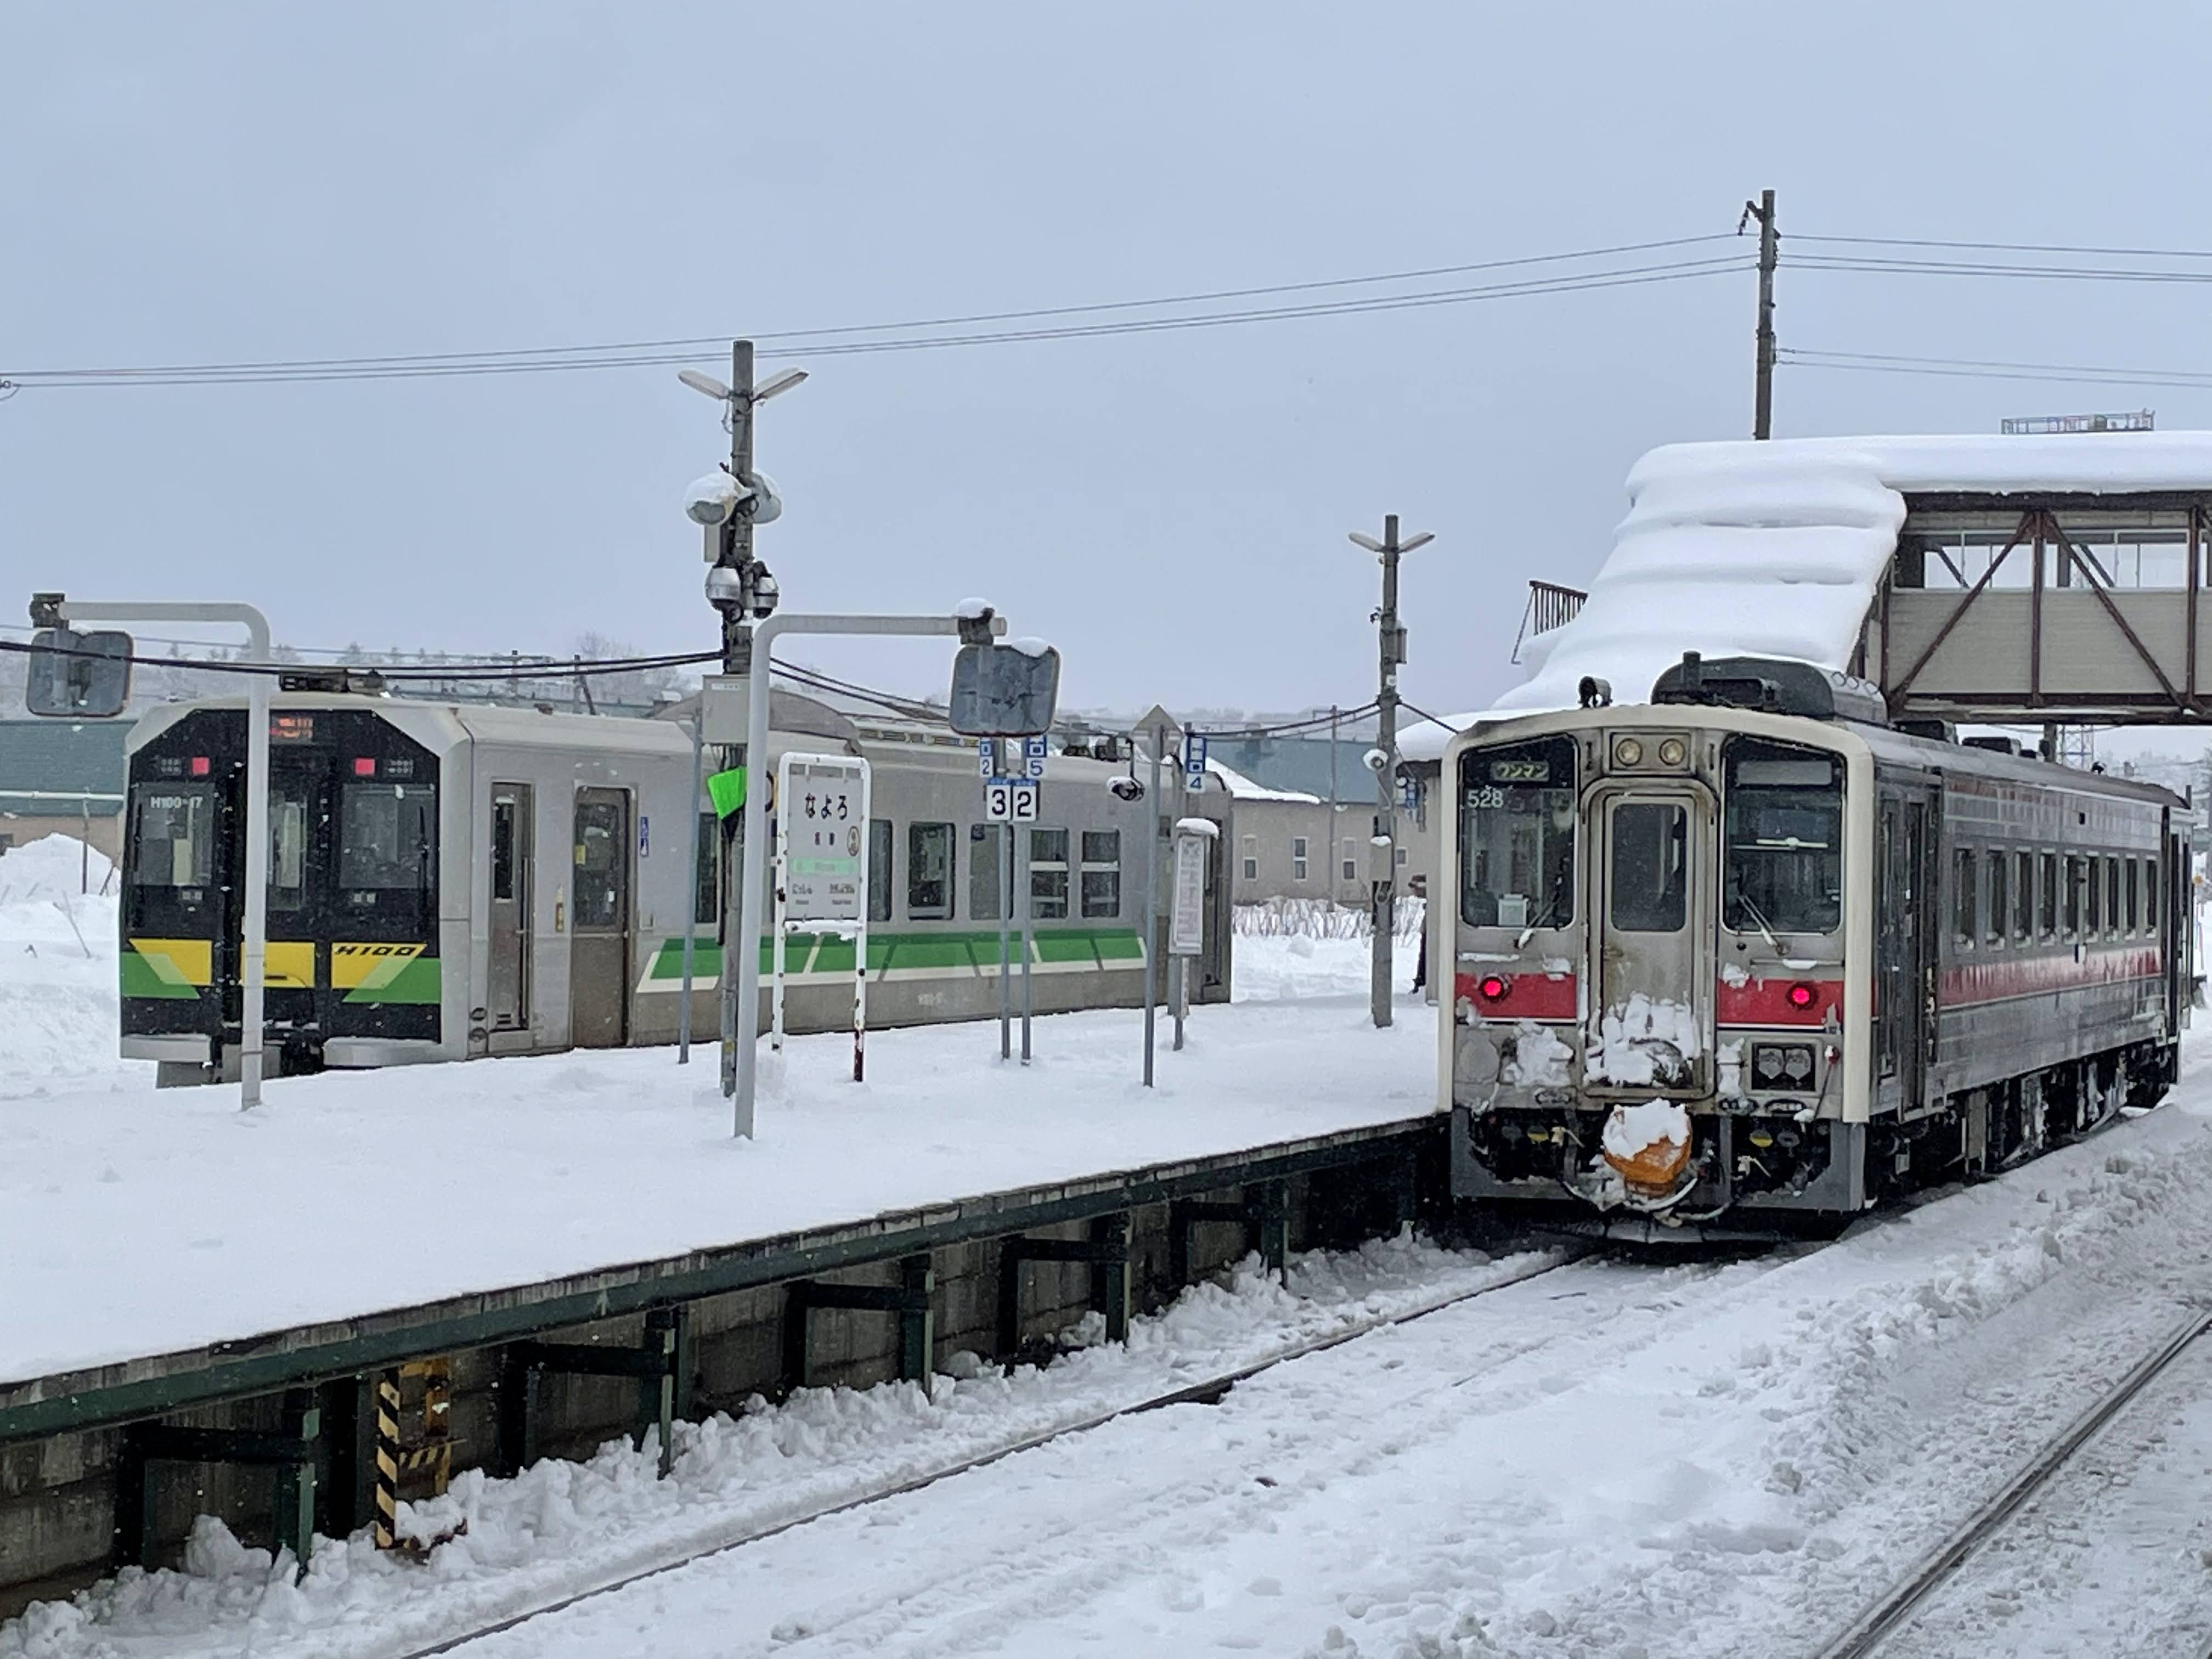
\includegraphics[width=\\linewidth]{image2.png}
    \caption{電車の画像の識別}
  \end{minipage}
  \hfill
  \begin{minipage}[t]{0.3\\textwidth}
    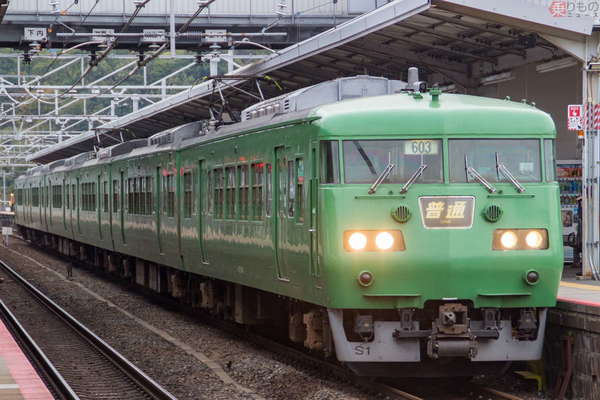
\includegraphics[width=\\linewidth]{image3.png}
    \caption{電車の動画の識別}
  \end{minipage}
\end{figure}
